\chapter{Dokumentacja biblioteki}
\label{app:docs}
\section{Przykład użycia}

\definecolor{mygreen}{rgb}{0,0.6,0}
\definecolor{mygray}{rgb}{0.5,0.5,0.5}
\definecolor{mymauve}{rgb}{0.58,0,0.82}

\lstset{%
  basicstyle=\footnotesize\ttfamily,%
  keywordstyle=\bfseries\color{green!40!black},%
  commentstyle=\itshape\color{purple!40!black},%
  identifierstyle=\color{blue},%
  stringstyle=\color{orange},%
  breakatwhitespace=false,         % sets if automatic breaks should only happen at whitespace
  breaklines=true,                 % sets automatic line breaking
  captionpos=t,                    % sets the caption-position to bottom
  frame=single,	                   % adds a~frame around the code
  keepspaces=true,                 % keeps spaces in text, useful for keeping indentation of code (possibly needs columns=flexible)
  language=C,                 % the language of the code
  rulecolor=\color{black}         % if not set, the frame-color may be changed on line-breaks within not-black text (e.g. comments (green here))
}

W~tabeli \ref{tab:sample-usage} przedstawiono przykład użycia biblioteki. W~przykładzie założono istnienie funkcji \texttt{RNG} służącej generowaniu losowych danych oraz~funkcji \texttt{network\_read} oraz~\texttt{network\_write}, które~odpowiednio odczytują i~wysyłają dane z~i~do sieci.

\captionof{table}{Przykład użycia biblioteki}
\label{tab:sample-usage}
\begin{lstlisting}
#include <seconn.h>

struct seconn sconn;

int c_seconn_write_data(void *src, size_t bytes) {
    return network_write(src, bytes);
}

void c_seconn_data_received(void *src, size_t bytes) {
    /*
     * src contains decrypted and authenticated data from other node that for
     * example could be shown to user
     */
}

void c_seconn_state_changed(seconn_state prev, seconn_state cur) {
    if(cur == AUTHENTICATED) {
        /*
         * sconn.public_key now contains authenticated public key of other
         * node. It's the best place to show it to user and ask for confirmation
         * that this is a~correct key.
         */
    }
}

int main() {
    // initialize sconn struct
    seconn_init(&sconn, c_seconn_write_data, c_seconn_data_received,
                c_seconn_state_changed, &RNG, 0);

    // fetch local public key, for example to show it to user
    uint8_t pubkey[64];
    seconn_get_public_key(&sconn, pubkey);

    // read data from network
    char buffer[64];
    unsigned bytes_read;
    while((bytes_read = network_read(buffer, bytes_read)) > 0) {
        // and pass it to seconn library.
        // seconn library will call functions passed to seconn_init if required
        seconn_new_data(&sconn, buffer, bytes_read);
    }
}
\end{lstlisting}
\FloatBarrier

\addtocounter{section}{1}
\addcontentsline{toc}{section}{\protect\numberline{\thesection}Dokumentacja Doxygen}
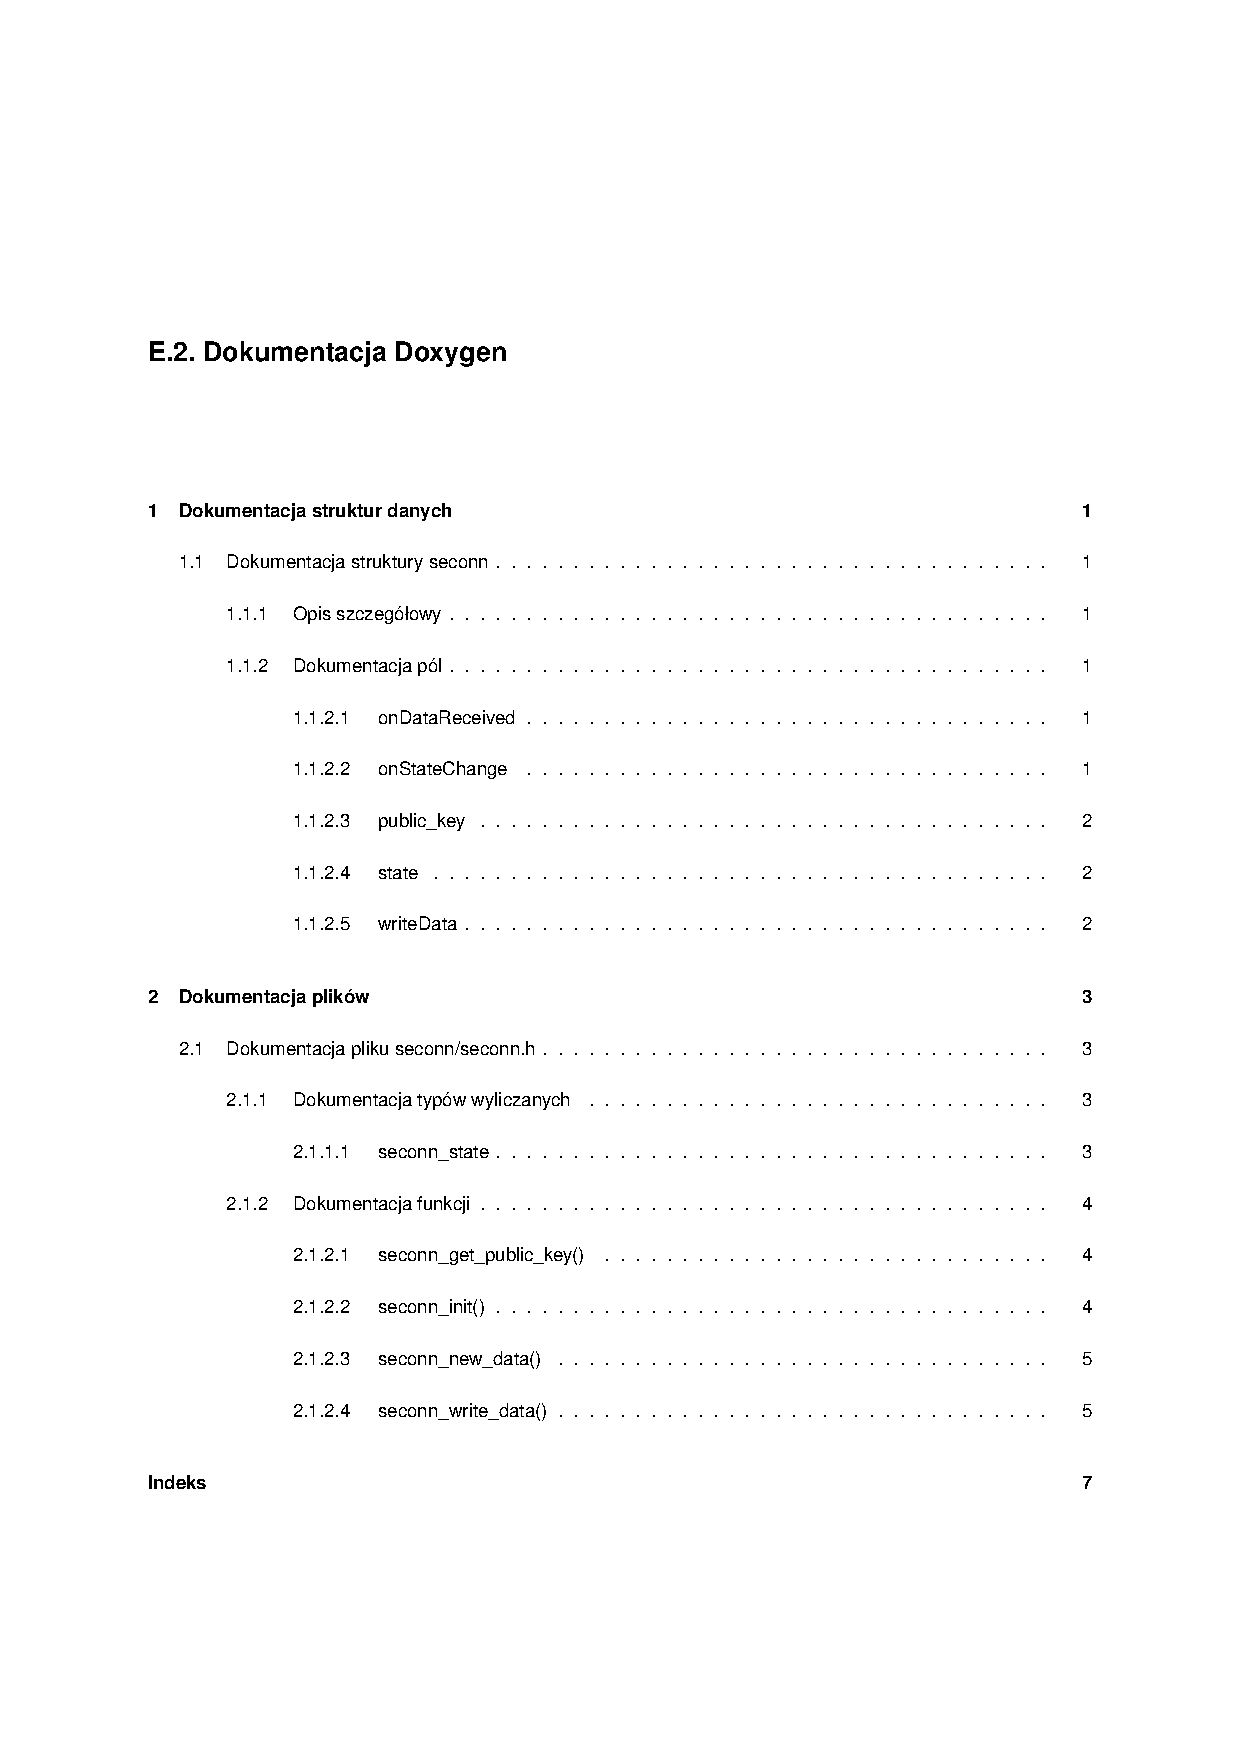
\includepdf[pages=-]{doxy.pdf}
